\chapter{Кинематический и силовой расчёт механизма привода}

\section{Техническое задание}

Дано:
\begin{itemize}
    \item вид передачи: червячная;
    \item момент на выходном валу: $T_2 = 21~Н \cdot м$;
    \item угловая скорость выходного вала: $\omega_2 = 18~с^{-1}$;
    \item передаточное число: $u = 10$.
\end{itemize}

Задача: рассчитать червячную передачу с заданными параметрами.

\section{Решение}
\begin{wrapfigure}{l}{0.35\textwidth}
    \begin{center}
        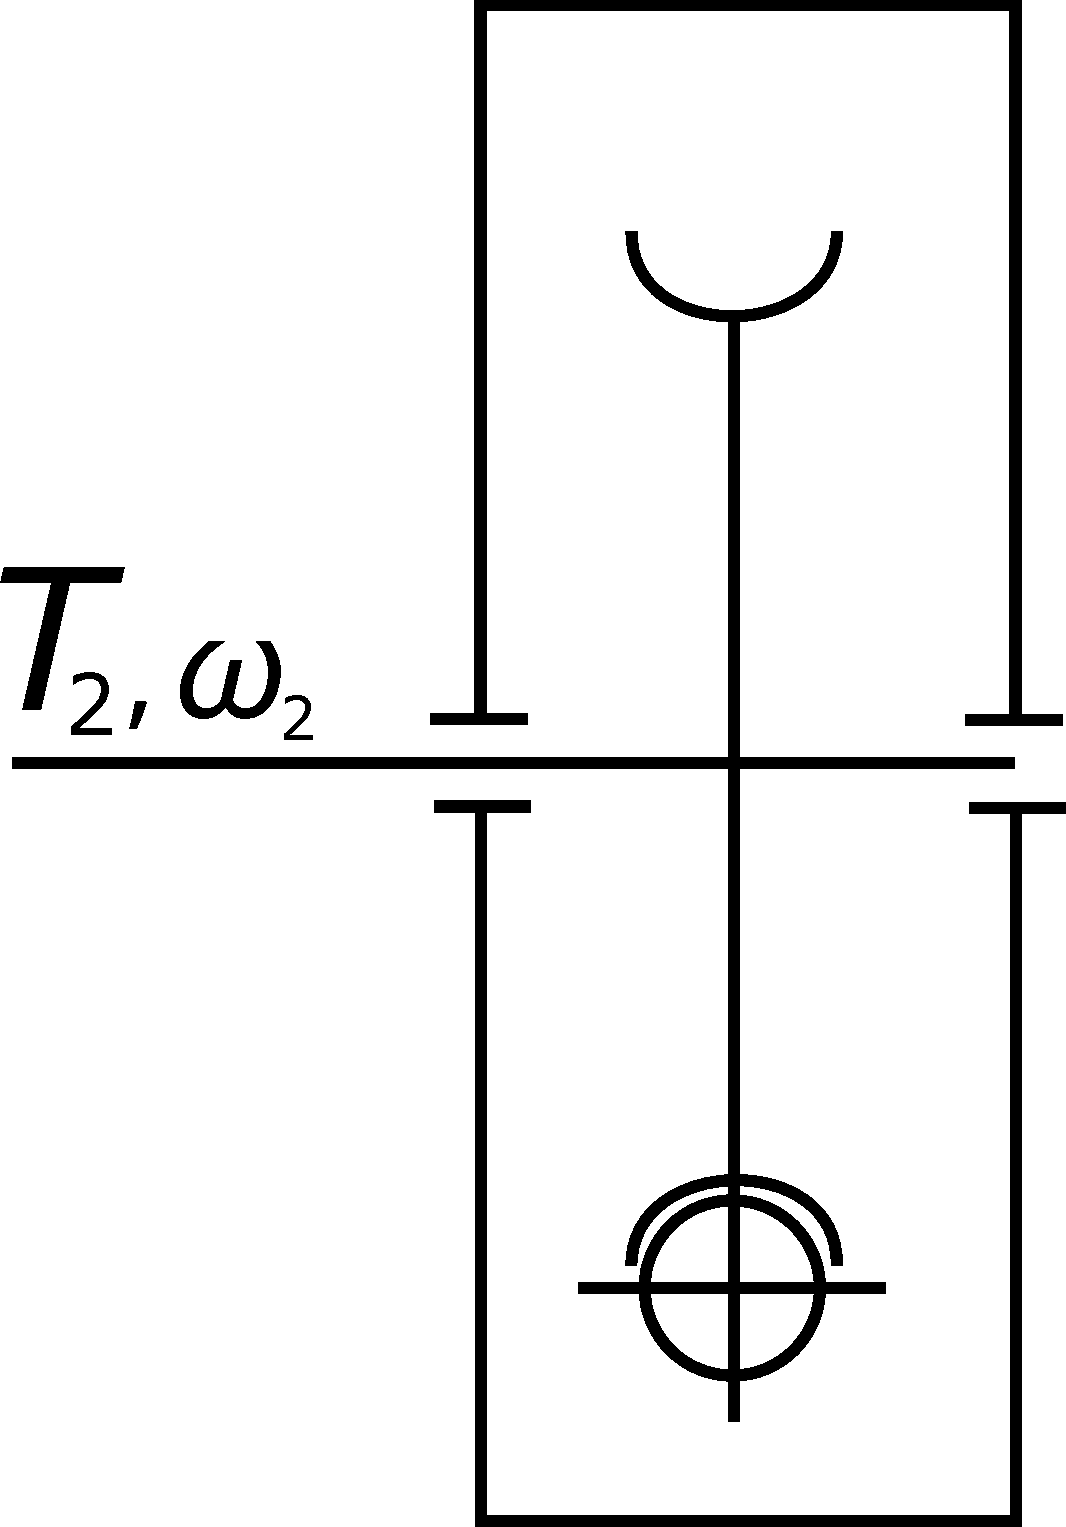
\includegraphics[width=\linewidth]{worm-drive}
        \caption{Кинематическая схема червячной передачи}
        \label{fig:worm-drive}
    \end{center}
\end{wrapfigure}

1. Назначаем число заходов червяка $z_1$ в зависимости от передаточного числа и требований к КПД механизма (табл.~\ref{tab:mechs}). Принимаем $z_1 = 4$.

2. Определяем число зубьев червячного колеса:
\[
    z_2 = z_1 u = 4 \cdot 10 = 40.
\]

3. Уточняем передаточное число:
\[
    u' = \frac{z_2}{z_1} = \frac{40}{4} = 10
\]
и определяем погрешность
\[
    \Delta u = \frac{u - u'}{u} \cdot 100~\%
             = \frac{10 - 10}{10} \cdot 100~\%
             = 0~\%.
\]
Погрешность не превышает допустимое значение в 5 \%.

4. Выбираем материалы червяка и червячного колеса.
Для уменьшения трения в зацеплении материалы червяка и червячного колеса должны составлять антифрикционную пару.
Для червяка применяем сталь 45, термообработка "--- улучшение; для червячного колеса "--- бронзу.
Марку бронзы выбираем в зависимости от скорости скольжения, которую ориентировочно принимаем
\[
    v_\text{ск} = 0.01 \omega_1 = 0.01 \omega_2 u = 0.01 \cdot 18 \cdot 10 = 1.8~м/с.
\]

При окружных скоростях до 5 м/с применяем алюминиево-железистую бронзу БрАЖ~9\==4 (по ГОСТ 18175-78).
Определяем допустимые контактные $\sigma_{HP}$ и изгибные $\sigma_{FP}$ напряжения для материала колеса при $v_{ск} = 2~м/с$, $\sigma_{HP} = 210~МПа$, $\sigma_{FP} = 80~МПа$.

\begin{table}[h!]
    \centering
    \caption{Значения КПД и передаточных чисел для механизмов и их элементов}\label{tab:mechs}
    \begin{tabular}{|l|l|m{7em}|m{7em}|m{7em}|m{7em}|}
        \hline
        \multicolumn{2}{|c|}{\multirow{2}{10em}{Передача, кинематическая пара}} & \multicolumn{2}{c|}{КПД ($\eta$)}         & \multicolumn{2}{c|}{Передаточное число ($u$)} \\ \cline{3-6} 
        \multicolumn{2}{|c|}{}                                                  & Закрытое исполнение & Открытое исполнение & Среднее          & Максимальное               \\ \hline
        \multirow{3}{*}{Червячная при}                & z = 1                   & 0.7 - 0.75          & -                   & 28--80           & 120                        \\ \cline{2-6} 
                                                      & z = 2                   & 0.75 - 0.82         & -                   & 14--40           & 40                         \\ \cline{2-6} 
                                                      & z = 4                   & 0.87 - 0.92         & -                   & 7--20            & 20                         \\ \hline
    \end{tabular}
\end{table}

5. Назначаем коэффициент диаметра червяка $q = 16$.

6. Определяем межосевое расстояние червячной передачи по условию контактной прочности зубьев червячного колеса, округлив результат до целого числа:
\[
    a_w \ge 306 \left(\frac{z_2}{q} + 1\right) \root 3 \of {\frac{T_2 K}{\left(\frac{z_2}{q}\right)^2 \cdot \sigma_{HP}^2}}
        = 306 \left(\frac{40}{16} + 1\right) \root 3 \of {\frac{21 \cdot 1.2}{\left(\frac{40}{16}\right)^2 \cdot 210^2}}
        = 49~мм,
\]
где $K = 1.2$ "--- коэффициент нагрузки.

7. Вычисляем основной модуль
\[
    m = \frac{2a}{q + z_2}
      = \frac{2 \cdot 49}{16 + 40}
      = 1.75~мм
\]
и округляем его до ближайшего большего значения по ГОСТ 19036-73 и проверяем, соответствует ли предварительно выбранный $q$ данному модулю. Принимаем $m = 2~мм$, $q = 16$.

8. Уточняем межосевое расстояние:
\[
    a_w = \frac{m (q + z_2)}{2}
        = \frac{2 (16 + 40)}{2}
        = 56~мм.
\]

9. Определяем делительные диаметры червяка и колеса:
\begin{align*}
    & d_1 = m q   = 2 \cdot 16 = 32~мм; \\
    & d_2 = m z_2 = 2 \cdot 40 = 80~мм.
\end{align*}

10. Определяем окружную скорость червяка при $\omega_1 = 180~м/с$:
\[
    v_1 = \frac{\omega_1 d_1}{2000}
        = \frac{180 \cdot 32}{2000}
        = 2.88~м/с.
\]

11. Определяем угол подъёма винтовой линии червяка:
\[
    \gamma = \arctg \frac{z_1}{q}
           = \arctg \frac{4}{16}
           \approx 14\degree 2'
\]

12. Вычисляем скорость скольжения в зацеплении:
\[
    v_{ск} = \frac{v_1}{\cos \gamma}
           = \frac{2.88}{\cos 14\degree 2'}
           = \frac{2.88}{0.998}
           \approx 2.89~м/с.
\]

13. Определяем КПД червячной передачи:
\[
    \eta = \frac{\tg \gamma}{\tg (\gamma + \rho)},
\]
где $\rho = \arctg f$ "--- угол измерения, $f$ "--- коэффициент трения в зацеплении, значение которого находим в зависимости от скорости скольжения, равный $f = 0.04\==0.05$ при $v_{ск}~=~2.89~м/с$.

Коэффициент трения принимает меньшее значение при шлифованном червяке.
При венце колеса из безоловянистой бронзы табличные значения следует увеличить на 30\==50~\%, т.е. $f = 0.04 \cdot 1.4 = 0.056$, а $\rho \approx 3\degree 12'$.  

Имеем
\[
    \eta = \frac{\tg 14\degree 2'}{\tg (14\degree 2' + 3\degree 12')}
         = \frac{0.25}{0.31}
         \approx 0.8
         = 80~\%.
\]

14. Определяем усилия в зацеплении:
\begin{itemize}
    \item окружное на колесе и равное ему осевое на червяке:
        \[
            F_{t2} = F_{a1}
                   = \frac{2000 \cdot T_2}{d_2}
                   = \frac{2000 \cdot 21}{80}
                   = 525~Н;
        \]
    \item радиальное ($\alpha = 20\degree$ "--- угол зацепления):
        \[
            F_{r2} = F_{r1}
                   = F_{t2} \tg \alpha
                   = 525 \cdot 0.364
                   \approx 191.1~Н
        \]
    \item осевое на колесе и равное ему окружное на червяке:
        \[
            F_{a2} = F_{t1}
                   = F_{t2} \tg \gamma
                   = 525 \cdot 0.250
                   \approx 131.2~Н
        \]
\end{itemize}

15. Назначаем восьмую степень точности передачи.
Уточняем коэффициент рассчётной нагрузки $K = K_\beta K_\nu$.
Ввиду хорошей прирабатываемости червячной пары коэффициент концентрации нагрузки $K_\beta$ принимаем равным единице.
Коэффициент динамичности $K_\nu$ зависит от степени точности передачи и скорости скольжения.
Для восьмой степени точности передачи при малой скорости скольжения $\nu_{ск} = 2.89~м/с$, $K_\nu = 1.2$.

16. Проверяем действительные значения контактных напряжений на рабочей поверхности зубьев червячного колеса:
\[
    \sigma_H = \frac{5400}{\cfrac{z_2}{q}} \sqrt{\frac{\left(\cfrac{z_2}{q} + 1\right)^3}{a_w^3} T_2 K_\beta K_\nu}
             = \frac{5400}{\cfrac{40}{16}} \sqrt{\frac{\left(\cfrac{40}{16} + 1\right)^3}{56^3} \cdot 21 \cdot 1 \cdot 1.2}
             \approx 169.4~МПа.
\]

17. Определяем запас контактной прочности:
\[
    n_H = \frac{\sigma_{HP}}{\sigma_H}
        = \frac{210}{169.4}
        \approx 1.24.
\]

18. Определяем геометрические параметры червячной передачи:
\begin{itemize}
    \item делительный параметр
        \begin{itemize}
            \item червяка: $d_1 = m q = 2 \cdot 16 = 32~мм$;
            \item колеса: $d_1 = m z_2 = 2 \cdot 40 = 80~мм$;
        \end{itemize}
    \item диаметр вершин зубьев
        \begin{itemize}
            \item червяка: $d_{a1} = d_1 + 2m = 32 + 2 \cdot 2 = 36~мм$;
            \item колеса: $d_{a2} = d_2 + 2m = 80 + 2 \cdot 2 = 84~мм$;
        \end{itemize}
    \item диаметр впадин
        \begin{itemize}
            \item червяка: $d_{f1} = d_1 - 2.4 m = 32 - 2.4 \cdot 2 = 27.2~мм$;
            \item колеса: $d_{f2} = d_2 - 2.4 m = 80 - 2.4 \cdot 2 = 75.2~мм$;
        \end{itemize}
    \item наружный диаметр
        \begin{itemize}
            \item червячного колеса
                \[
                    d_{am2} \le d_{a2} + \frac{6m}{z_1 + 2}
                            = 84 + \frac{6 \cdot 2}{4 + 2}
                            = 86~мм;
                \]
        \end{itemize}
    \item длина нарезанной части червяка:
        \[
            b_1 \ge (12.5 + 0.09 z_2) m
                = (12.5 + 0.09 \cdot 40) \cdot 2
                = 32.2~мм 
        \]
        (принимаем $b = 34~мм$);
    \item ширина колеса:
        \[
            b_2 \le 0.67 d_{a1}
                = 0.67 \cdot 36
                = 24.12~мм
        \]
        (принимаем $b_2 = 24~мм$);
    \item угол охвата червяка колесом:
        \[
            \sin \delta \le \frac{b_2}{d_{a1} - 0.5m}
                        = \frac{24}{36 - 0.5 \cdot 2}
                        = 0.686,
        \]
        откуда $\delta \le 43\degree 18'$ (принимаем $\delta = 43\degree$);
\end{itemize}

18. Проверяем напряжение изгиба в зубьях червячного колеса:
\[
    \sigma_F = 0.7 Y_F \frac{F_{t2} K_\beta K_\nu}{b_2 m \cos \gamma} \le \sigma_{FP},
\]
где $Y_F = 1.38$.

При
\[
    z_v = \frac{z_2}{\cos^3 \gamma}
        = \frac{40}{\cos^3 14\degree 2'}
        = \frac{40}{0.970^3}
        = 43.8
\]
(принимаем $z_v = 44$) получаем следующее значение напряжения:
\[
    \sigma_F = 0.7 \cdot 1.38 \cdot \frac{525 \cdot 1 \cdot 1.2}{24 \cdot 2 \cdot \cos 14\degree 2'}
             \approx 13~МПа;
\]

Имеем
\[
    \sigma_F = 13 < \sigma_{FP} = 80.
\]
Запас изгибной прочности
\[
    n_F = \frac{\sigma_{FP}}{\sigma_F} = \frac{80}{13} \approx 6.15.
\]

